%%%%%%%%%%%%%%%%%%%%%%%%%%%%%%%%%%%%%%%%%%%%%%%%%%%%%%%%%%%%%%%%%%%%%%%%%
% This file is part of the LaTeX sources of the OMDoc 1.2 specifiation
% Copyright (c) 2006 Christoph Lange
% This work is licensed by the Creative Commons Share-Alike license
% see http://creativecommons.org/licenses/by-sa/2.5/ for details
\svnInfo $Id: main.tex 6161 2006-10-03 13:04:46Z  $
\svnKeyword $HeadURL: https://svn.omdoc.org/repos/omdoc/branches/omdoc-1.2/doc/spec/projects/swim/main.tex $
%%%%%%%%%%%%%%%%%%%%%%%%%%%%%%%%%%%%%%%%%%%%%%%%%%%%%%%%%%%%%%%%%%%%%%%%%

\section{{\swim} -- An OMDoc-based Semantic Wiki}
\begin{project}{swim}{http://kwarc.eecs.iu-bremen.de/projects/swim}
\pauthors{Christoph Lange\and Michael Kohlhase}
\pinstitute{Computer Science, International University Bremen}
\end{project}

{\swim} is a semantic wiki for collaboratively building, editing and browsing a
mathematical knowledge base of {\omdoc} theories. Our long-term objective is to develop a
software that facilitates the creation of a shared, public collection of mathematical
knowledge and serves work groups of mathematicians as a tool for collaborative development
of new theories.  Even though the work reported here was initially motivated by solving
the MKM author's dilemma~\cite{KohKoh:cdad04}, we contend that the new application area
MKM can also contribute to the development of semantic wikis.

Technically, {\swim} is based on the semantic wiki engine
\scsys{IkeWiki}~\cite{schaffert06:ikewiki}, which was chosen because of its
modular design, its rich semantic web infrastructure, its user assistance for
annotations, and its orientation towards
learning~\cite{schaffert06:learning-with-semantic-wikis}.

\subsection{Semantic Wikis}

A wiki~\cite{LeuCun01:wikiway} is a web server
application that allows users to browse, create, and edit hyperlinked pages in a web
browser, usually using a simple text syntax.  In contrast to most content management
systems, wiki pages are accessible via an URL containing their title.  A new page can be
created by linking from an existent page to the page to be created.  This link will then
lead to an edit form.  Usually, anyone is allowed to edit pages on a wiki, but access can
be restricted.  Other characteristics of wikis include permanent storage of old page
versions (with facilities to display differences between two versions and to restore a
certain version), notification about recent changes, and full-text search.

Semantic
wikis~\cite{voelkel06:semanticwikistateoftheart,TolPas06:wikis-semantic-hypermedia}
enhance wikis by Semantic Web technologies, such as {\rdf}~\cite{LasSwi:rdf99} or
ontologies.  Usually one page represents one concept from a real-world domain, which has a
type, possibly some metadata, and typed links to other concepts.  For example, a link from
a wiki page about ``Life, the Universe and Everything'' to another page about Douglas
Adams could be typed as ``is author of''.  In terms of {\rdf}, this can be expressed by the
following subject--predicate--object triple,

\[
(\mbox{``Douglas Adams''},\;\mbox{isAuthorOf},\;\mbox{``Life, the Universe and
Everything''})
\]

where the \textit{isAuthorOf} relation would be defined in an ontology.  These links are
usually displayed in a navigation box next to the page contents. Semantic wikis only deal
with wiki text, not with mathematics, though some allow to embed mathematical formulae as
presentational-only {\TeX}.

{\swim} encourages users to collaborate: Non-mathematicians can collaborate in creating a
``Wikipedia of mathematics'' by compiling the knowledge available so far, while scientists
can collaboratively develop new theories.  Users get an immediate reward for many of their
contributions: Once they specify the type of a page or relations of one page to another,
this information will be displayed in a box of navigation links.  We intend to make the
data created in {\swim} usable for external services by offering an export facility for
{\omdoc} documents and by integrating them into {\swim}.  Mathematicians developing
theories will be assisted to retain an overview of theory dependencies in order not to
break them.  Social software services will further utilize the semantic information
available from the theories and from tracking the user interaction log (``Who did what on
which page when?'').  User feedback to pages can be extended to social bookmarking, which
is ``the practice of saving bookmarks [of Internet resources] to a public web site and
`tagging' them with keywords.''~\cite{lomas05:social-bookmarking} The more users tag a
certain resource, the higher a social bookmarking service will rank it.

The enhancements of the data model semantic wikis bring along --- compared to traditional
wikis --- are already present in the {\omdoc} format, so that an {\omdoc}-based wiki only
needs to operationalize their underlying meaning. For example, typed links, which are
implemented via an extension to the wiki syntax in \scsys{Semantic
  MediaWiki}~\cite{voelkel06:semanticwikipedia} or editable through a separate editor in
\scsys{IkeWiki}~\cite{schaffert06:ikewiki}, are implemented by means of the \texttt{for}
attribute to {\omdoc}'s elements (e.g.\ \texttt{<example for="\#id-of-assertion">}).
{\swim} makes them editable easily and visualizes them adequately.  A semantic wiki
targeted at mathematics must ensure that dependencies between concepts are preserved.
Results in this area will be interesting for non-mathematical semantic wikis as well,
especially when they support higher levels of formalization such as ontologies.

\subsection{Design of {\swim}}

\subsubsection{Concepts and Relations}

The smallest unit that can be displayed, edited, linked to, or archived in a wiki is a
page. In a semantic wiki, it usually describes one {\emph{concept}}, including its
properties and its relations to other concepts.  While standalone {\omdoc} documents can
contain more than one theory, is is important to keep pages small in a wiki to improve the
effectivity of usage.  Furthermore, usual semantic wikis only store and display metadata
and typed links per page; {\swim} does too.\footnote{Semantic information will only be
  considered on the theory and statement levels of {\omdoc} --- directly or through
  reasoning in the case of transitive closures ---, not on the object level.}  Users are
strongly encouraged to define at most one theory per wiki page and to roll out
non-constitutive statements (see {\mysecref{statements-constitutive}}) to separate pages,
referencing their context theory.  As constitutive statements cannot exist without an
enclosing theory, but as, on the other hand, we want each wiki page to form a valid
document, we introduced a new element {\element[ns-elt=swim]{page}}, which can be a child
of an {\element{omdoc}} element and which has the same content model as a
{\element{theory}} element --- in particular, it can hold several theory-constitutive
statements and connect them to their context theory.
\begin{wrapfigure}{r}{8cm}
  \begin{tikzpicture}[scale=1.5,thin,font=\sffamily,>=triangle 60]
    \tikzstyle{concept}=[font=\sffamily\bfseries,draw,minimum height=3.5ex,rounded corners]
    \tikzstyle{every path}=[font=\small\sffamily];
    \node[concept] (t) at (0,1) {theory};
    \node[concept,dashed] (s) at (0,0) {\itshape statement};
    \node[concept] (d) at +(-158:2.0cm) {definition};
    \begin{scope}[shift={(d)}]% control point for e->d
      \coordinate (da) at +(-90:1.5cm);% relative to s, not to a!
    \end{scope}
    \node[concept] (a) at +(-120:1.5cm) {assertion};
    \begin{scope}[shift={(a)}]% control point for e->a
      \coordinate (aa) at +(-30:1cm);% relative to s, not to a!
    \end{scope}
    \node[concept] (p) at +(-60:1.5cm) {proof};
    \node[concept] (e) at +(-22:2.0cm) {example};
    \draw[->] (t.-60) .. controls +(-60:0.5cm) and +(-30:0.5cm) .. node[right]
    {imports} (t.east);
    \draw[->] (s) -- node[left] {context for} (t);
    \draw[-open triangle 60] (d) -- node[above] {is a} (s);
    \draw[-open triangle 60] (a) -- node[above left] {is a} (s);
    \draw[-open triangle 60] (p) -- node[above right] {is a} (s);
    \draw[-open triangle 60] (e) -- node[above] {is a} (s);
    \draw[->] (p) -- node[above] {proves} (a);
    \draw[->] (e) ..
    controls +(-120:1cm)
    and (aa) ..
    node[below left] {exemplifies} (a);
    \draw[->] (e) ..
    controls +(-90:1.5cm)
    and (da) ..
    node[below left] {exemplifies} (d);
  \end{tikzpicture}
  \caption{Subset of {\omdoc}'s system ontology}\vspace*{-.5cm}
\end{wrapfigure}
{\omdoc}'s system ontology has been partly coded in OWL-DL and imported to the wiki's {\rdf}
store, which is implemented using the Jena Semantic Web Framework for
Java~\cite{URL:jena:web}. Theories as well as statements of any type form concepts, and
the most important relations between those concepts are extracted from the {\omdoc} pages
on saving and then stored as {\rdf} triples.  These relations include:
\begin{itemize}
\item The import relation between theories
\item The relation of a statement to its context theory
\item The relation of an example to the statement it exemplifies
\item The relation of a proof to the assertion it proves
\end{itemize}
It is planned to also take relations given by user interaction into consideration, such as
``Who edited which page when?'', and to combine ontology-defined relations and user
relations.  For example, a metric estimating the {\emph{degree of difficulty}} of a page,
calculated by counting the questions on the discussion page, could be implemented.
Furthermore, the user can specify taxonomic relations, which cannot be stated explicitly
in {\omdoc}, such as (``all differentiable functions are continuous''), as annotations in
an ontology language like {\rdf} Schema or {\owl}.

\subsubsection{User Interface and Interaction Model}

Pages can be rendered to XHTML plus presentational MathML using the transformations
described in {\mychapref{transform-xsl}}. There is also a browsable source code view, which is
useful for documents that are not written in textbook style.

Not only will the user be able to navigate along the dependency graph, she will also be
able to {\emph{interact}} with the system: she will be asked whether she wants to explore
the theories required as dependencies in further detail.

Suppose that the user is currently reading the page containing the theory {\snippet{ring}}
from the elementary algebra example from {\mychapref{dg-elal}}. In this case the wiki will
not only display navigation links to the direct dependencies {\snippet{group}} and
{\snippet{monoid}}, but it will also provide unobtrusive buttons that allow the user to
give one of the commands in {\myfigref{gui-showdeps}}. Not only the last case will be
recorded --- the others are interesting as well for \emph{social bookmarking}.  For
example, if many users requested a theory $t$ to be explained, the system could default to
display not only the direct dependencies but also the level-two dependencies, for it seems
that $t$ is too difficult for only being explained shallowly.

\begin{myfig}{gui-showdeps}{The command buttons to navigate along the dependencies}
  \begin{minipage}{8cm}
\begin{description}
\item[{\bf{No, thanks!}}] ``{\emph{I already know group and monoid.}}''
\item[{\bf{Explain}}] ``{\emph{Please show me group and monoid, I want to learn about
      ring's prerequisites.}}'' --- group and monoid will be displayed.
\item[{\bf{Explore}}] ``{\emph{Please show me {\emph{all}} prerequisites for ring.}}'' ---
  group, monoid, and semigroup, are opened in separate windows or serialized into one
  page.
\item[{\bf{Suspend}}] ``{\emph{I want to know about group and monoid, but only later.}}''
  --- {\swim} keeps a notice in the user's profile that she wants to read group and monoid
  sometime.  Reminder links to suspended theories are shown on a separate navigation bar.
\end{description}
\end{minipage}\quad
\begin{minipage}{2.5cm}
  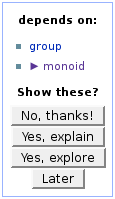
\includegraphics[width=2.5cm]{projects/swim/gui-showdeps}
\end{minipage}
\end{myfig}

\subsubsection{Further work}

Further work on {\swim} will concentrate on integrating a lightweight
management of change process.  Second, while the wiki is yet a user-friendly
\emph{browser}, there is still a demand for assisting users to \emph{edit}
{\omdoc}.  To this end, the {\qmath} preprocessor (see {\mysecref{qmath}}) will
be integrated into {\swim}.  Mathematical objects entered as {\qmath} will be
kept in this syntax for display in the edit form, but they will be converted to
{\omdoc} for rendering for presentation and when pages are exported to another
application.

%%% Local Variables: 
%%% mode: stex
%%% TeX-master: "../../omdoc"
%%% End: 

% LocalWords:  matwebsearch Ioan Sucan nC dx dy dt runningex XPointer ns attr
% LocalWords:  mq anyorder xmlns domainofapplication bvar ci cn eq OAI API da
% LocalWords:  Lange CPoint wikis dateness parseable isAuthorOf MediaWiki omdoc
% LocalWords:  aa wiki's Wiki wiki IkeWiki JA hypermedia elt semithick pres dg
% LocalWords:  elal gui showdeps qmath stex metadata wiki's scheint mir kein zu
% LocalWords:  Gegensatz sein
